\begin{problem}{/images/problems/26_oppenheimer.jpg}{Oppenheimer ticket queue}
40 people are standing in a line in front of a cinema to buy tickets to the Oppenheimer movie. The ticket price is 5 dollars. Out of these 40 people, 25 of them have only 5 dollar bills and 15 of them have only 10 dollar bills. The cashier has no cash in the beginning, however, when people start purchasing tickets she will collect cash based on what they give her. Indeed, the price of the ticket is 5 dollars and if a person gives a 10 dollar bill to the cashier, she has to return a 5 dollar bill. How many different permutations of people will allow the cashier to always give a 5 dollar bill to the people who only have 10 dollar bills?\\[0.2cm]

Link to the problem on Twitter:  \url{https://twitter.com/Riazi_Cafe/status/1691691003118596147}\end{problem}
\begin{solution}
The correct answer is $
(\binom{40 }{25} - \binom{40}{26}) \cdot 25! \cdot 15!$.\\[0.2cm]

Let $m$ be the number of people who have $5$ dollar bills and $n$ be the number of people who have $10$ dollar bills.
We show the configuration of a permutation of the people in the queue with a diagram similar to the one below, where we start from the origin and if the next person has $5$ dollar bills, we go to the top right, and if he only has $10$ dollar bills, we go to the bottom right.

In order to keep the diagram small, instead of $m=25$ and $n=15$ for the main problem,  we show an example diagram for  $m=6$ and $n=4$. 

\begin{center}
	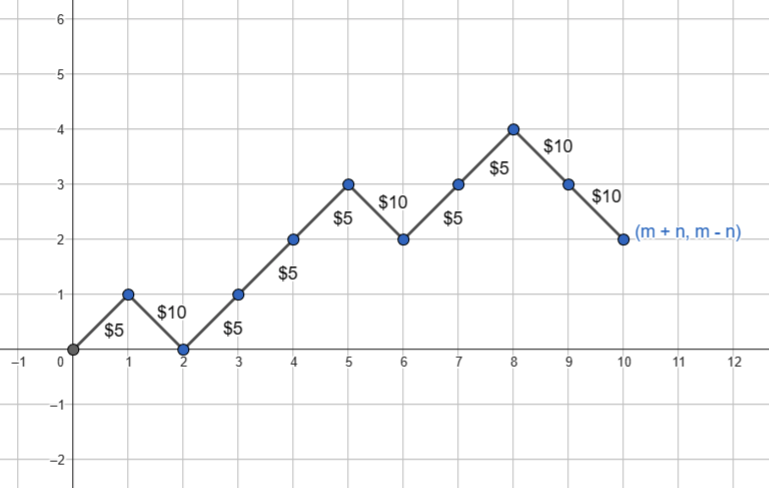
\includegraphics[width=9cm]{/images/problems/26_diagram1.png}
\end{center}

The number of such graphs is ${n+m \choose m}$. Notice that a configuration is acceptable, only if we never go below line $y=0$. An example of an unacceptable configuration is given below.

\begin{center}
	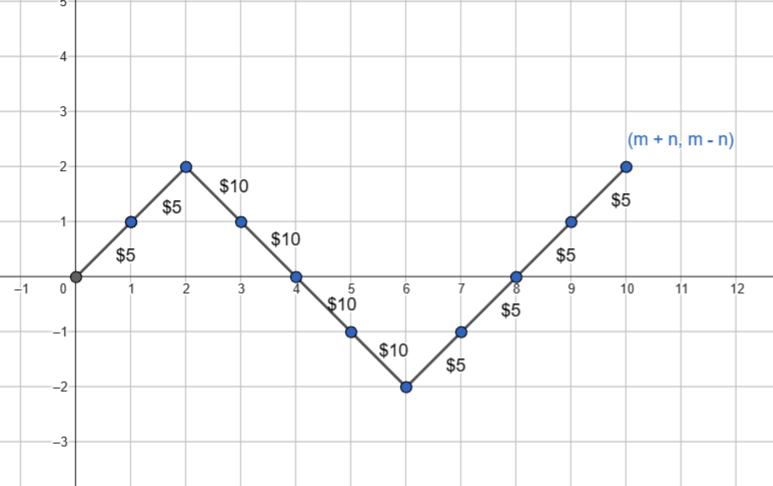
\includegraphics[width=9cm]{/images/problems/26_diagram2.png}
\end{center}

To count these unacceptable configurations, we observe that these states are the states where the graph intersects the line y=-1. We show a 1-to-1 mapping between such figures and the ones that start from location $(0,-2)$. To this end, we mirror the graph before the first intersection with line $y=-1$. For example, for the figure above the result would be as follows:

\begin{center}
	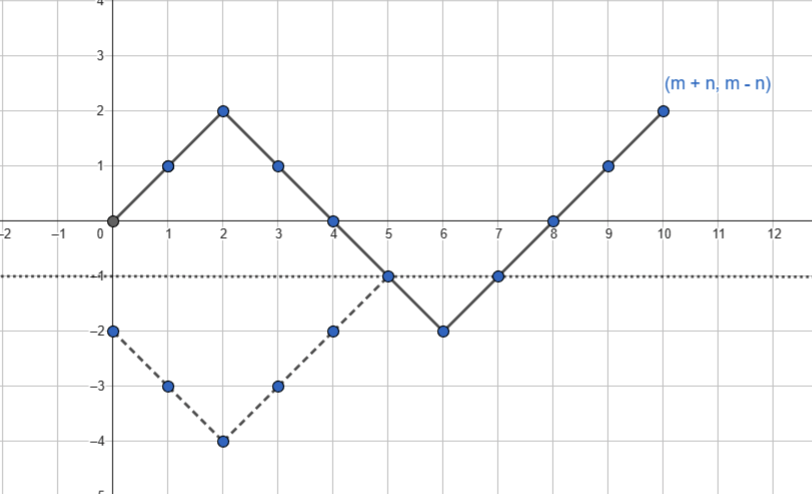
\includegraphics[width=9cm]{/images/problems/26_diagram3.png}
\end{center}

Notice that in all such graphs we start from point $(0,-2)$ and end at $(m+n, m-n)$ as before. These diagrams have a one-to-one correspondence with unacceptable states. Thus, the number of such configurations is to ${n+m \choose m+1}$.

So the total number of acceptable configurations is equal to ${n+m \choose m} - {n+m \choose m+1}$. In these configurations, we are indifferent between people who have the same set of bills.
If we also take into account such distinctions, the answer would be the following:

$$
({n+m \choose m} - {n+m \choose m+1}) \times n! \times m!
$$



\end{solution}
